% \section{Introduction}
% As the field of therapeutic interventions has developed, music therapy has become a potent tool for treating a variety of psychological and emotional illnesses. \citep{americanmusictherapyassociation_2005_what}
% It is acknowledged as a clinical and evidence-based practice. Without demanding musical proficiency from participants, it strives to improve mental, emotional, physical, and cognitive abilities in a variety of contexts, including schools, mental health centers, hospitals, and nursing homes. \citep{clevelandclinic_2020_music}
% Scientific research suggest that novel activities such as vibroacoustic treatment, improvisation, singing popular songs, and composing can support personal growth and healing. \citep{craig_2019_what}
% As a result, music therapy is a very flexible and successful therapeutic approach. 
% Its effectiveness stems from its ability to recognize and address each individual's emotional condition. 
% This idea aligns with the potential of face expression recognition technologies.

% \gls{fer} technology bridges the gap between emotional understanding and technological innovation.
% It is a sophisticated version of facial recognition that uses \gls{ai} and \gls{ml} to identify human emotions through facial expressions.
% Based on feature analysis, \gls{fer} could identify emotions like happiness, sadness, anger and neutral. \citep{huang_2023_a}
% The ability to sense and react to individual emotional states makes it valuable in the healthcare sector, where it has the potential to transform patient care through monitoring emotional health, diagnosing illnesses and enabling more personalized treatment plans.
% Particularly in therapy, it provides a non-invasive way to gauge patient's emotional states which allows therapists to more precisely customize their approaches. \citep{zharovskikh_2020_how}

% Building upon these foundational technologies, music recommendation systems represent another pivotal element in personalizing therapy sessions. 
% These systems make music recommendations based on a number of variables, including user preferences, behavior, psychographic traits, and demographics. 
% Additionally, it will categorise listeners into several groups such as savants, enthusiasts, causals and in differents, for more efficient tailoring in order to improve listening experiences. \citep{song_2012_a}
% Since music has a enormous effect on emotional and psychological health, these systems' accuracy becomes especially important in therapy. \citep{schedl_2021_music}
% Innovatively, \gls{ai}-driven models have pushed the boundaries further by detecting patient's real-time emotions, and offering recommendations that not only match but also influence mood and psychological states. \citep{babu2023emotionaware}
% Technology plays a vital role in augmenting music's therapeutic potential, as evidenced by the introduction of \gls{ai} into music recommendation systems, which bring in a new era of tailored therapy encounters.

% \section{Music Therapy}
% The history and theoretical foundations of music therapy track back thousands of years, but the field's practical development really took off in the 1940s.
% Following World War II, the US War Department published Technical Bulletin 187 in 1954 that detailed a program for rehabilitating service members through music. \citep{else_2014_music}
% With its emphasis on the use of music in a range of therapeutic settings, this curriculum established a standard for the official acknowledgement and advancement of music therapy as a profession.
% The \gls{namt} was founded in 1950, which further cemented the path for the formal recognition and advancement of music therapy as a profession. \citep{else_2014_music}
% During this crucial time, the field of music therapy had substantial growth and advocacy, which resulted in the development of standards for training and application. 
% The field then united to establish the \gls{amta} in 1998. \citep{else_2014_music}
% \\
% \indent The theoretical foundations of music therapy are as varied and deep as its history, encompassing a wide range of psychological theories and studies such as developmental psychology, psychoanalysis, and John Bowlby's attached theory. \citep{ackerman_2018_what}
% These theories shows how music might be used therapeutically to promote safe attachments, improve social and emotional growth, and assist dynamic, patient-centered therapy. 
% The improvisational methods developed by Kenneth Bruscia place an additional emphasis on creativity and spontaneity, which facilitate the use of music to convey feelings and build interpersonal bonds.\citep{bruscia_1987_improvisational}
% \\
% \indent Furthermore, empirical studies and neuroscientific discoveries that demonstate the effects of music on emotional regulation, stress response, and neuroplasticity reinforce the foundation of music therapy. \citep{hillecke_2005_scientific}
% According to this research, music therapy can benefit a wide range of people, including trauma survivors and infants. It also highlights the benefits of music therapy for mental health and cognitive development.
% \\
% \indent Music therapy's adaptability and relevance are highlighted by the inclusion of early educational programs and advocacy in addition to focused interventions for military groups. \citep{else_2014_music}
% According to Gooding and Langston (2019), music therapy has proven to have a deep ability to adapt to changing healthcare needs and societal demands as evidenced by its supportive role in post-war recovery from conditions such as \gls{ptsd} and \gls{tbi} \nocite{gooding_2019_music}, and its acceptance as a clinical profession. \citep{garrison_2021_music}
% With a strong foundation in evidence-based treatment and a profound comprehension of music's therapeutic potential, music therapy has come a long way from mystical conceptions to a scientifically validated practice.

% \section{Facial Emotion Recognition}

% \section{Music Recommendation System}
\subsection{Introduction of Music}
The development of human communication and social cohesiveness is closely linked to the origins of music. 
Protohumans probably created the first musical sounds through rhythmic awareness and vocalizations with variable pitch before musical instruments were invented. 
Primitive humans showed the ability to compose music even before they learned to speak. 
The development of early human civilizations may have benefited from this musical talent by fostering social cohesion and collaboration.
\\
\indent The comparison of early speech or the pitched sounds of animals to historical music demonstrates how primitive music was as a medium of expression before sophisticated language. 
A tight relationship exists between the growth of rhythmic awareness and the capacity to produce percussion sounds and the formation of music in the evolutionary timeline.
The ability to perceive and produce music was probably important for social interactions when Homo neanderthalensis and Homo sapiens evolved.
One major explanation for the evolution of music is the innate human desire to collaborate and form social contexts for doing so. 
Early human society appears to have relied heavily on music, judging from its role in fostering social cohesiveness, entertaining, enabling dance, and supporting ritualistic behaviors.
\\
\indent Essentially, the origins of music can be found in the basic human urge for collaboration, socialization, and the development of cultural contexts that support these endeavors. 
Even in its most primitive incarnations, music influenced human communities and may have helped Homo sapiens outperform other hominid species in terms of cultural development.

\subsection{Evolution and Diversity of Music}
\begin{figure}[!ht]
    \centering
    \subfloat[\centering Cuneiform Alphabet \\Image from \cite{a2021_how} \label{subfig:cuneiform}]{{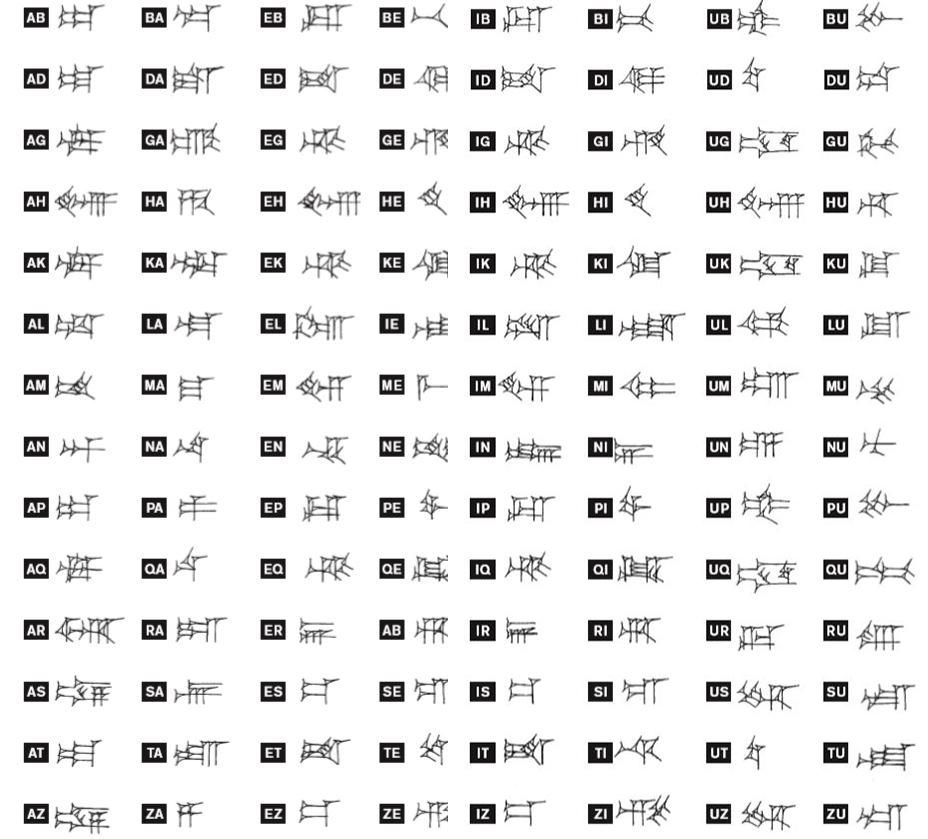
\includegraphics[width=5cm]{Images/cuneiform.jpg}}}%
    \qquad
    \subfloat[\centering World's Earliest Music Composition \\Image from \cite{porter_2018_did} \label{subfig:first_song}]{{
\includegraphics[width=5cm]{Images/first_song.jpg}}}%
\end{figure}
The history of music is extensive and ancient, and it is an essential part of human culture. 
In Syria, a cuneiform "alphabet" (\ref{sub@subfig:cuneiform}) containing the earliest known written composition of music was found (\ref{sub@subfig:first_song}) \cite{porter_2018_did}.
It is thought to have been composed some 3400 years ago. 
The oldest musical instruments, according to archaeological evidence, date back approximately 40,000 years, but the history of music is far older still \cite{killin_2018_the}.
Despite not yet being documented in the archaeological record, these instruments offer a window into far older musical endeavors. 
Proto-musical evolution most likely started about 400,000 years ago, based on the social brain hypothesis \cite{dunbar_social_brain}. 
Musical traditions developed further as people left Africa and spread over the world, reaching a turning point during the Holocene. 
This historical voyage demonstrates the persistent and varied impact that music has played in human history.
Moving forward, there are so many types of music, each representing unique expression of culture, emotion and creativity:
\begin{itemize}
    \item \textbf{Classical Music}: a diverse and evolving tradition, extending beyond the commonly associated period of 1750 to 1820 and encompassing composers from Bach to contemporary artists. 
    It serves as a living and influential force in the world of music, shaping compositions for orchestras, chamber ensembles, solo performers, and even finding unexpected expressions in various genres, from video-game scores to popular music. \cite{gabler_2013_what} \nocite{pentreath_2022_why}
    \item \textbf{Jazz}: originating in early 20th-century New Orleans, is characterized by complex harmony, syncopated rhythms, and a focus on improvisation. 
    Emerging from a rich tradition of ragtime and blues, jazz evolved into a versatile genre that expanded its influence globally, encompassing popular music standards, modal music, and even avant-garde compositions.\cite{beek_2021_what}
    \item \textbf{Blues}: both a musical form and genre, initially associated with melancholy themes, has evolved to encompass a broader range of subjects and emotions, aiming to uplift through music.\cite{chaudhuri_2022_what}
    Characterized by specific chord progressions, a walking bass, call and response, and unique features like microtonality and flattened 'blue' notes, blues is known for its distinct sound and expressive style. \cite{bbc_2023_history}
    \item \textbf{Electronic}: utilizes diverse sound sources, ranging from recorded sounds captured by microphones to those generated by electronic oscillators and complex computer installations. 
    Typically played back through loudspeakers, electronic music can be created using various technologies, with the exception of "live electronic music," which involves real-time performance. \cite{hiller_2019_electronic}
    \item \textbf{Country}: originating in rural Southern and Western areas in the early 20th century, was initially labeled "hillbilly music" before adopting the official term "country and western music" in 1949. 
    Rooted in the ballads, folk songs, and popular tunes of English, Scots, and Irish settlers, country music gained commercial recognition in the early 1920s, marked by its realistic portrayal of rural life contrasting with the sentimental tone prevalent in popular music of that era. \cite{_2019_country} \nocite{_2021_country}
    \item \textbf{Hip-Hop}: a cultural movement that gained widespread popularity in the 1980s and '90s, serves as the foundational music for rap—a style featuring rhythmic and/or rhyming speech, which became the movement's enduring and influential art form. 
    Hip-hop, beyond its musical dimension, encompasses diverse elements such as graffiti art, breakdancing, and social activism, reflecting a multifaceted expression of urban culture and creativity. \cite{tate_2019_hiphop} \nocite{seanmccollum_2019_hiphop}
    \item \textbf{Rock}: a form of popular music that emerged in the 1950s and by the end of the 20th century became the dominant global music genre, influencing the recording industry, international retail, and radio and television playlists. 
    While dictionary definitions often focus on its strong beat and instrumentation, the cultural significance of rock lies in its social and ideological distinctions from other music genres, particularly its development as a term to distinguish certain attitudes and practices from those associated with pop music.\cite{frith_2018_rock}
\end{itemize}

\subsection{Music and Emotion}
Since ancient times, people have been fascinated by the paradoxical connection that exists between music and emotion.
Even though music is an abstract art form that appears to be removed from everyday life, it has a profound potential to evoke strong emotional responses.
This ability of music to trigger strong emotions is also demonstrated in other social circumstances, such as advertising. 
This encounter is further enhanced by the relationship that exists between music and our individual life experiences.
Emotions, influenced by these encounters, provide our perception and thought processes a personalized meaning that connects the abstract quality of music to the concrete events of our everyday life. 
This complex tapestry that highlights the profound influence of music on our emotional environment is created by the blending of music, emotion, and human experience \cite{juslin_2013_music}.
\\
\indent Numerous musical elements that have been thoroughly explored are combined to convey emotions through music. 
Pace, mode, harmony, interval, rhythm, sound level, timbre, timing, articulation, accents, tone attacks and decays, and vibrato are some of these characteristics. 
Emotion in music is expressed through compositional elements as well as performance elements. 
Still, it's not an easy task to express feelings through music. 
Certain musical elements can be employed to convey a range of moods, showing that certain elements are not always reliable predictors of a certain emotion. 
The Lens Model \cite{juslin_2013_music}, which characterizes emotional expression in music as involving probabilistic and partially redundant auditory cues, sheds more light on this complexity.
Listeners combine several cues for successful emotion recognition, and the redundancy of cues allows for a high level of emotion recognition through different combinations, offering room for creativity and personal expression \cite{pereira_2011_music}.
\section{Artificial Intelligence and Machine Learning}
\subsection{Artificial Intelligence}
\gls{ai} is a broad field that includes using technology to build machines and computers that can replicate cognitive abilities connected to human intellect. 
These abilities include making recommendations, language understanding, data processing, and visual perception.
\gls{ai} should be viewed as a group of technologies incorporated into systems rather than as a stand-alone system that can understand, learn, and respond to complex problems.

\subsection{Machine Learning}
\gls{ml} is a branch of \gls{ai} focused on enabling machines and systems to learn and enhance their performance through experience. 
Instead of relying on explicit programming, machine learning employs algorithms to analyze vast datasets, derive insights, and subsequently make informed decisions. 
These algorithms continually improve their performance as they are exposed to more data. The outcomes of this learning process are the machine learning models, which become more proficient with increased exposure to data.

\subsection{Machine Learning Algorithms}
\subsubsection{Linear Regression}
\nocite{mali_2021_linear}
\nocite{rohithgandhi_2018_introduction}
\nocite{kwiatkowski_2021_gradient,ibm_what}
\nocite{_2019_descending}
\gls{lr} is a supervised learning algorithm used to model the relationship between a dependent variable (target) and one or more independent variables (features).
The fundamental assumption of \gls{lr} is that there exists a linear relationship between the input variables and output. \cite{ibm_2022_about}
\begin{equation} \label{eq:linear_equation}
    y = mx + b
\end{equation}
\begin{equation} \label{eq:linear_regression}
    Y = \beta_0 + \beta_{1}X_{1} + \beta_{2}X_{2} + \cdots + \beta_{n}X_{n} + \epsilon
\end{equation}
\indent A \gls{lr} model can be represented by the equation \ref{eq:linear_regression} where $Y$ represented the dependent variable. 
$\beta_0$ is the y-intercept, $\beta_1, \beta_2, \cdots, \beta_3$ are the coefficients  and the $\epsilon$ is an error term, representing the unobserved factors that affect $Y$ but are not accounted for by the model.
The logic of it is same as Linear Equation (\ref{eq:linear_equation}) where using the gradient of the line ($m$), the value of $x$ and the y-intercept ($b$) to get the value of $y$, which is what we are trying to predict. 
\\
\begin{figure}[!ht]
    \centering
    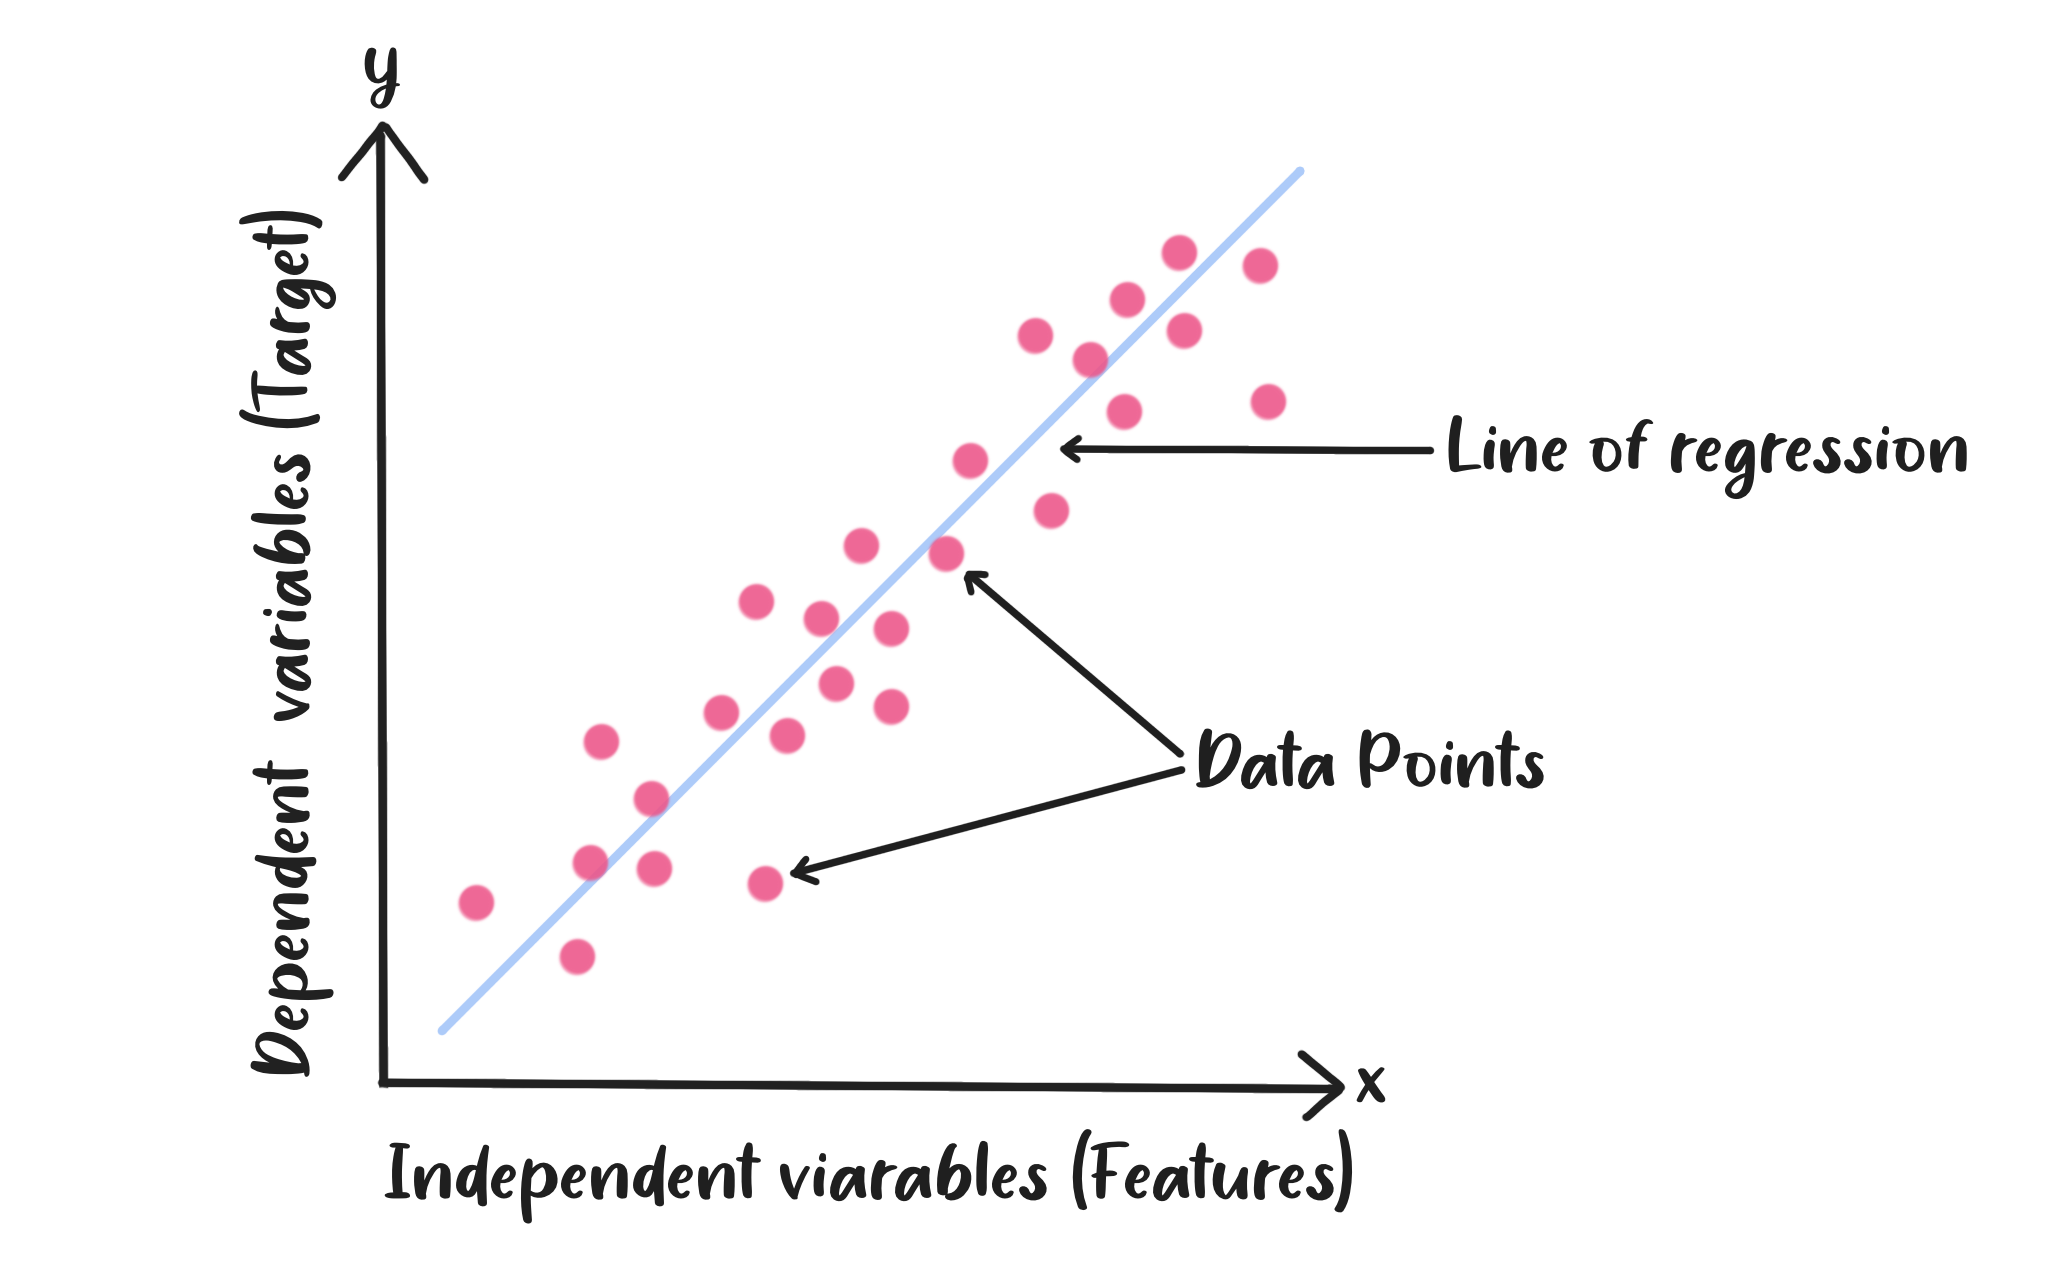
\includegraphics[width=10cm]{Images/lr.png}
    \caption{Linear Regression}
    \label{fig:lr}
\end{figure}
\\
\indent While using \gls{lr}, the main objective is to find the values of $\beta_0, \beta_1,...,\beta_n$ that minimize the error between the predicted value ($\hat{Y}$) and the actual value ($Y$) in the training data.
\\
\begin{equation} \label{eq:mse}
    \text{MSE} = \frac{1}{n} \sum_{i=1}^{n} (Y_i - \hat{Y}_i)^2
\end{equation}
\\
Therefore, \gls{mse}, a cost function to measures the average squared difference between $\hat{Y}$ and $Y$, is introduced to quantify the goodness of fit of the model to the training data. 
If the current result is not optimized, \gls{gd}, an optimization algorithm, will be used to adjust the coefficients, $\beta_0, \beta_1,...,\beta_2$, towards the direction that minimizes the \gls{mse} until it reach the convergence (Figure \ref{fig:gd}).
\\
\begin{figure}[!ht]
    \centering
    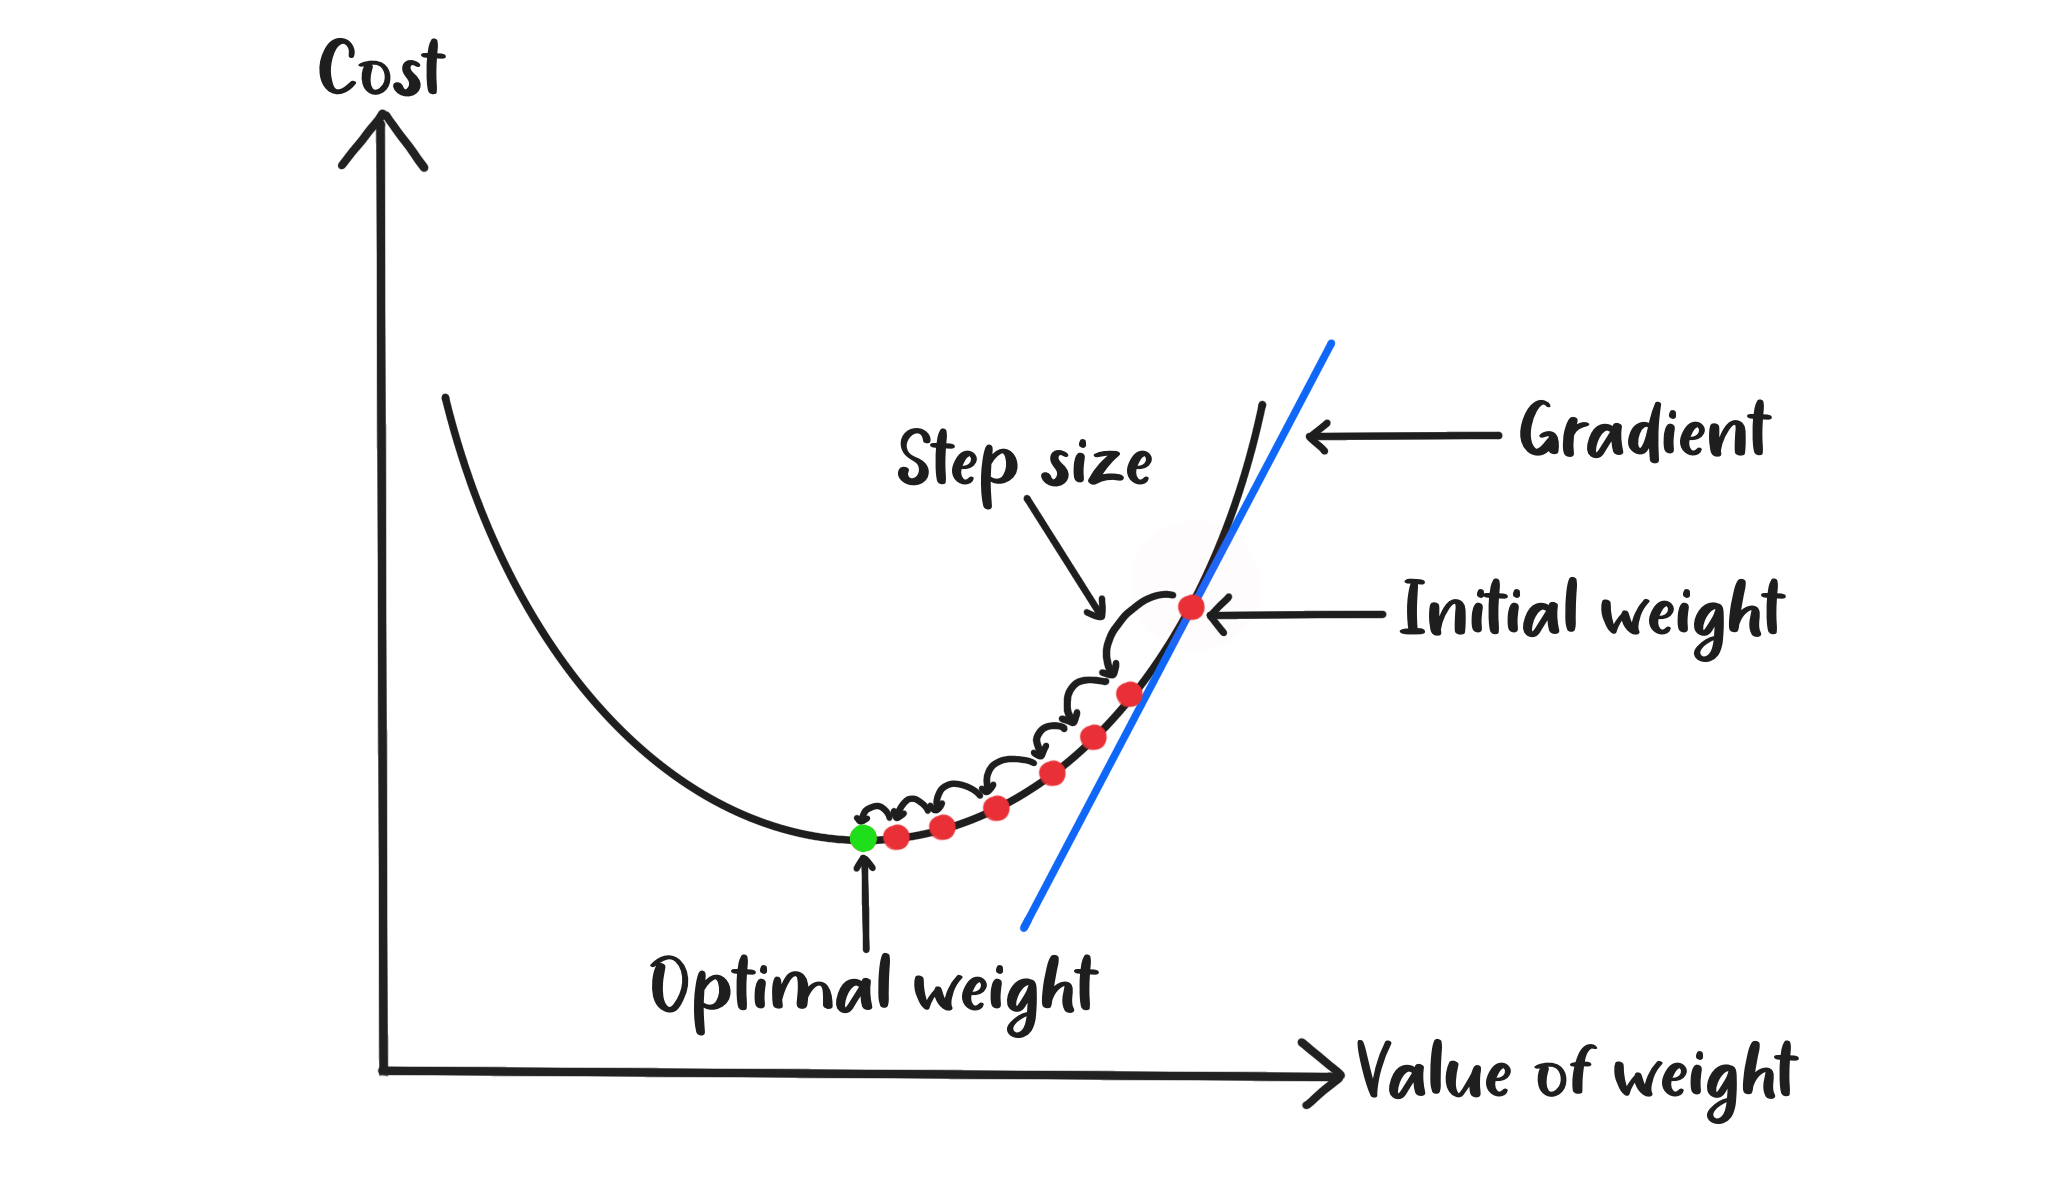
\includegraphics[width=10cm]{Images/gd.png}
    \caption{Gradient Descent}
    \label{fig:gd}
\end{figure}
\\
\subsubsection{Support Vector Machine}
\nocite{berwick_an}
\nocite{_14}
\nocite{saini_2021_support}
\gls{svm} is a supervised \gls{ml} algorithm where we used for classification, regression and outliers detection.
The main goal of it is to find the hyperplane that best separates the data into different classes based on statistical approaches. \cite{gron_2019_handson}
\\
\begin{figure}[!ht]
    \centering
    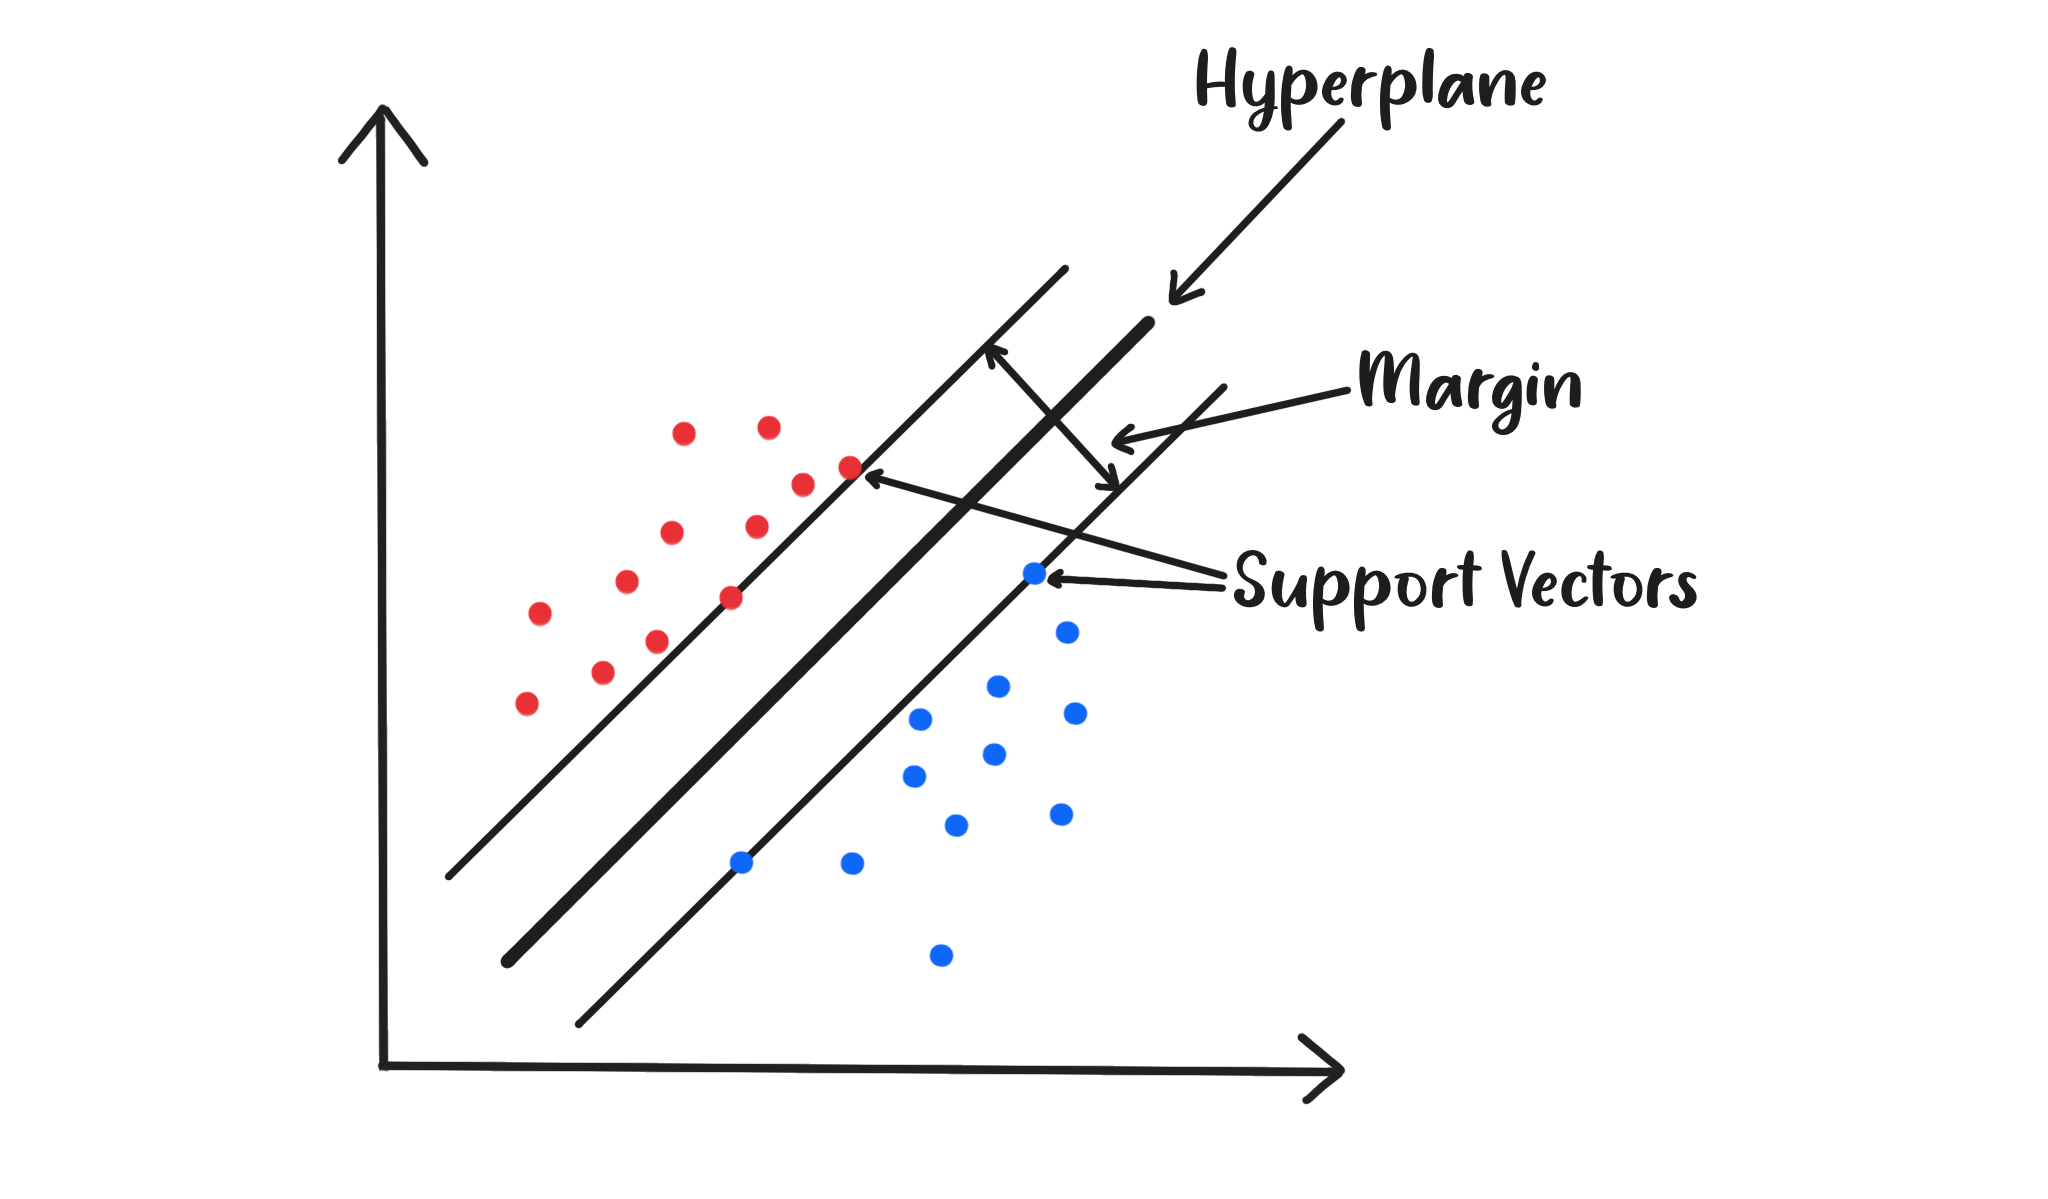
\includegraphics[width=10cm]{Images/svm.png}
    \caption{Support Vector Machine}
    \label{fig:svm}
\end{figure}
\\
\indent While using \gls{svm}, the greater the margin, the better the result would be as it has better generalization to new or unseen data. 
There are two types of \gls{svm} for classification, which are Linear \gls{svm} and Non-linear \gls{svm}.
A linear \gls{svm} finds the optimal hyperplane that maximizes the margin between classes for linearly separable data as Figure \ref{fig:svm}.
\\
\begin{equation} \label{eq:linear_svm}
    f(x) = \text{sign}(\mathbf{w} \cdot \mathbf{x} + b)
\end{equation}
\\
The decision function of linear \gls{svm} (Equation \ref{eq:linear_svm}) is used to defines the ability to classify data points into different classes.
When the result is greater than or equal to zero, the prediction would be positive. If $f(x)$ is less than zero, the decision function predicts the negative class. 
\begin{figure}[!ht]
    \begin{minipage}{0.45\linewidth}
        \begin{equation}
            f(x) = \text{sign}(\sum_{i=1}^{n} \alpha_{i}y_{i}K(x,x_{i}) + b) \label{eq:non_linear_svm}
        \end{equation}
    \end{minipage}
    \hfill
    \begin{minipage}{0.45\linewidth}
        \begin{equation}
            K(x,x_{i}) = (x \cdot x_{i} + c)^{d} \label{eq:poly_svm}
        \end{equation}
    \end{minipage}

    \begin{minipage}{0.45\linewidth}
        \begin{equation}
            K(x,x_{i}) = \text{exp}(-\frac{\parallel x - x_{i} \parallel ^ {2}}{2 \sigma ^ {2}}) \label{eq:rbf_svm}
        \end{equation}
    \end{minipage}
    \hfill
    \begin{minipage}{0.45\linewidth}
        \begin{equation}
            K(x,x_{i}) = \text{tanh}(\alpha x \cdot x_{i} + c) \label{eq:sigmoid_svm}
        \end{equation}
    \end{minipage}
\end{figure}
\\
\indent For non-linearly separable data, \gls{svm} uses kernel functions such as polynomial, sigmoid and radial basis function (RBF), to map the data into a higher-dimensional space where hyperplane can separate the classes.
The equation \ref{eq:non_linear_svm} is the decision function of non-linear \gls{svm}. 
The kernel function, denoted by $K(x,x_{i})$ in the equation, would be replaced by equation \ref{eq:poly_svm} if a polynomial kernel were used.
Similar with the other kernels, if the RBF kernel is employed, it would be exchanged with equation \ref{eq:rbf_svm}, and for sigmoid kernel, it would be replaced with equation \ref{eq:sigmoid_svm}.

\subsubsection{Random Forest}
\nocite{er_2021_random}
\nocite{scikitlearn_2018_sklearnensemblerandomforestclassifier}
\nocite{yiu_2019_understanding}
\gls{rf} is an ensemble learning algorithm that belongs to the family of decision tree-based methods.
A group of decision trees that have been trained on various dataset subsets make up the forest of \gls{rf}, and the final result is derived from averaging the predictions of each individual tree. \cite{ibm_2023_what}
\\
\begin{figure}[!ht]
    \centering
    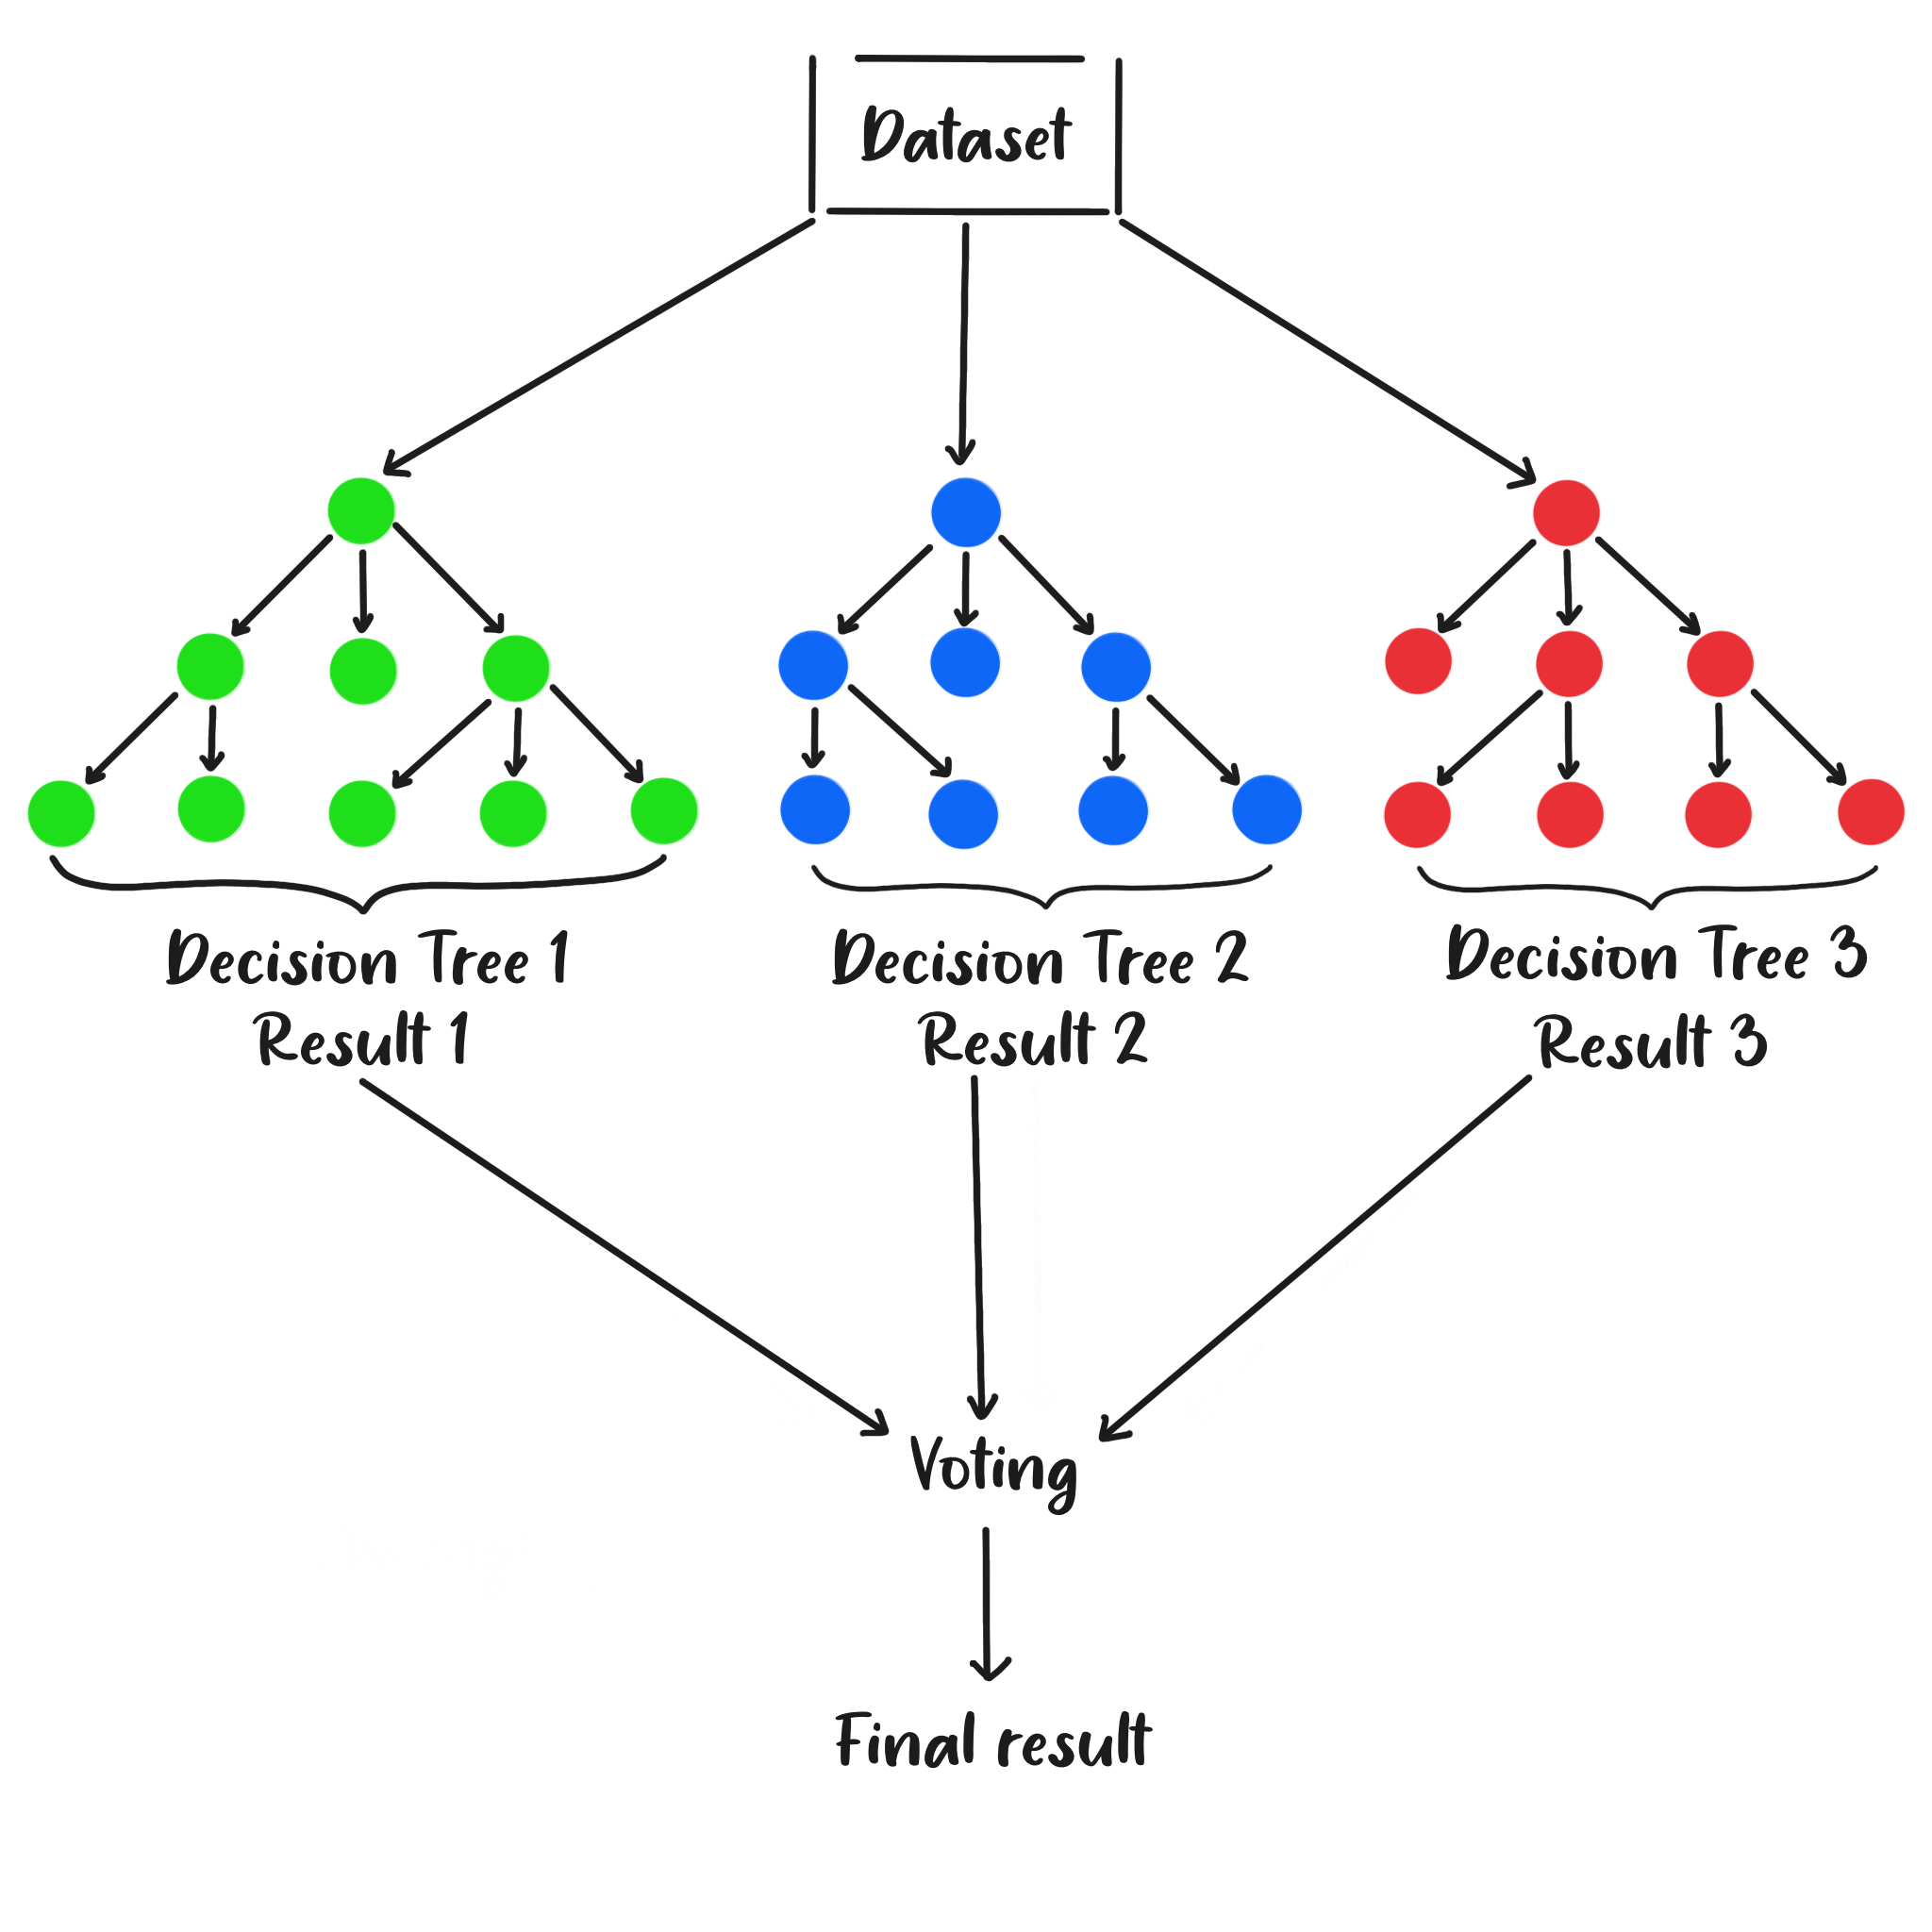
\includegraphics[width=10cm]{Images/rf.png}
    \caption{Random Forest}
    \label{fig:rf}
\end{figure}
\\
\indent As Figure \ref{fig:rf} shown, \gls{rf} builds multiple Decision Trees and combines them to get a more accurate and stable prediction than any individual model.
This process is called bagging which is one of a type of ensemble learning. 
In the process, the entire dataset is separated into subsets and each decision tree is trained individually on a subset that is selected at random.
This adds variety and unpredictability to the trees.
The training process will then generate results for each model, and the final output is determined by the "votes" for a class from each tree.
The class with the majority of votes is chosen as the final prediction.
\subsubsection{K-Nearest Neighbors}
\nocite{srivastava_2019_introduction}
\nocite{geeksforgeeks_2018_knearest}
\nocite{harrison_2018_machine}
\gls{knn} is a intuitive supervised machine learning method used for both classification and regression tasks. 
The main idea of \gls{knn} is to predict the label of new data point based on its k-nearest data points in the feature space. \cite{ibm_what_knn}
\\
\begin{figure}[!ht]
    \centering
    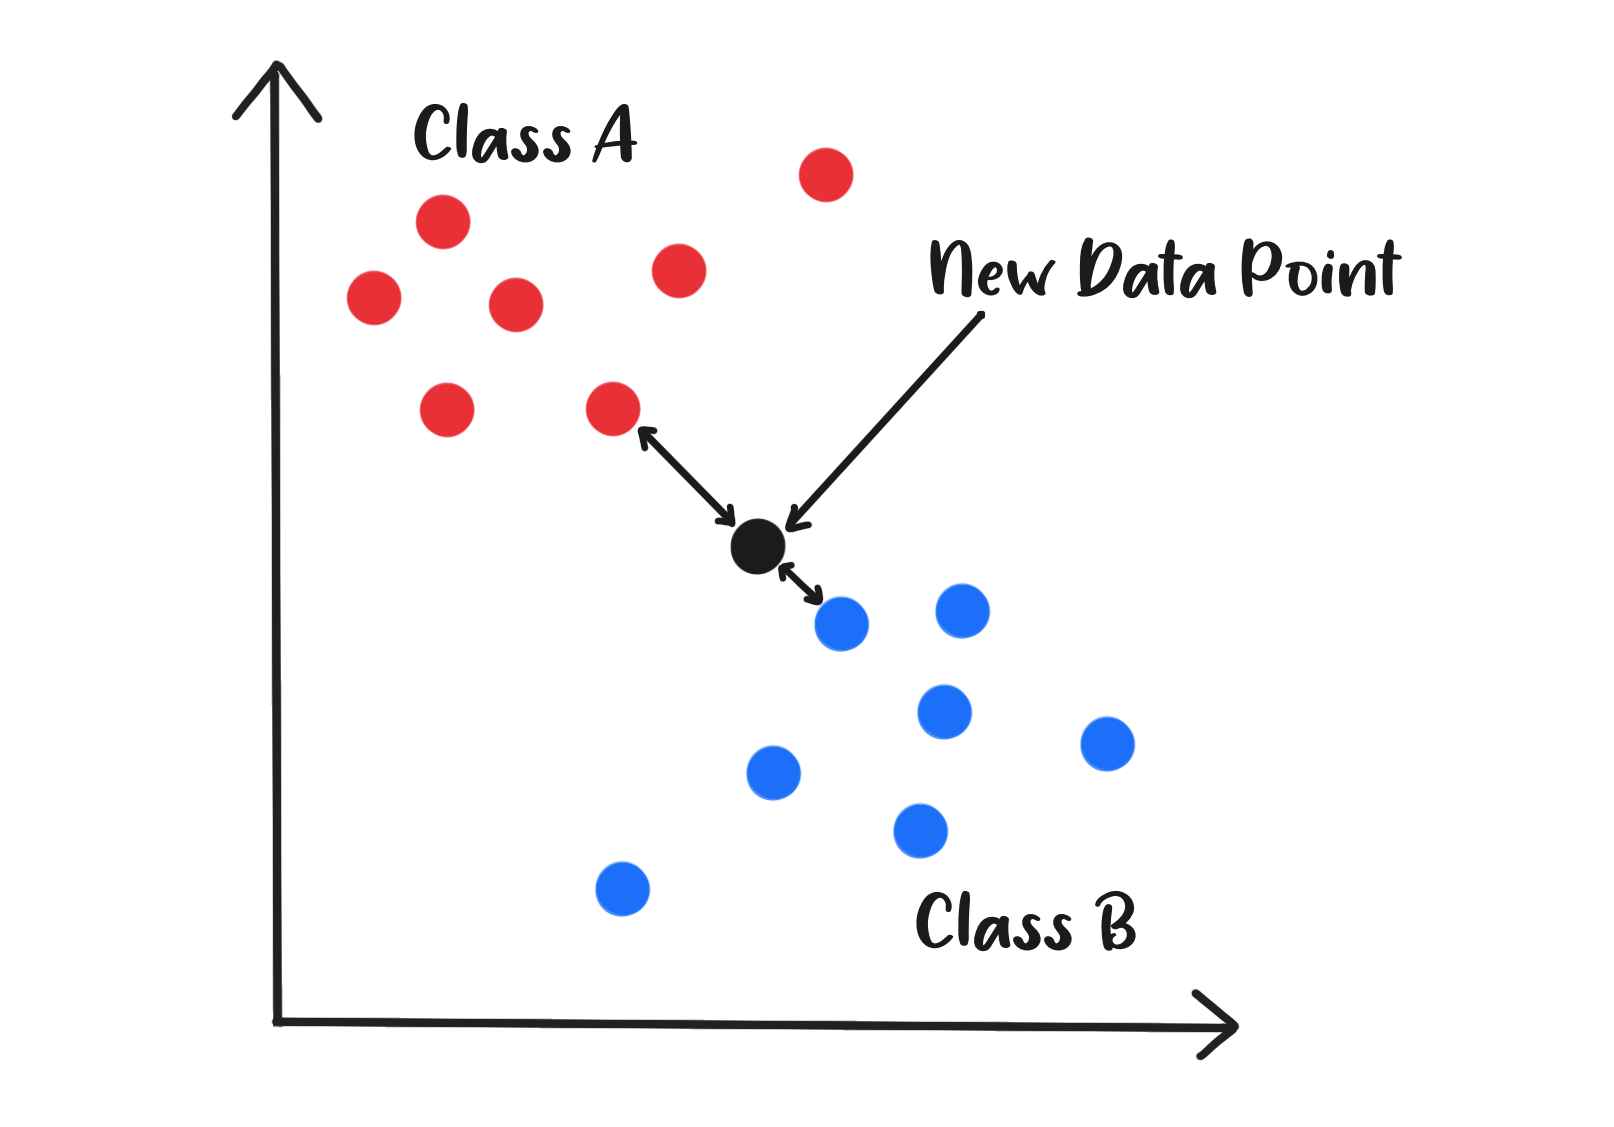
\includegraphics[width=10cm]{Images/knn.png}
    \caption{K-Nearest Neighbors}
    \label{fig:knn}
\end{figure}
\\
\indent \gls{knn} uses distance metric (Equation \ref{eq:euclidean}) to calculate how similar two data points are to one another.
\gls{knn} finds the k training data points that, according to the selected distance metric, are closest to a given data point.
In classification tasks, the majority class among a new data point's k-nearest neighbors predicts the class that the data point will fall into.
\\
\begin{equation} \label{eq:euclidean}
    d(P,Q) = \sqrt{\sum_{i=1}^{n}(p_{i} - q_{i})^{2}}
\end{equation}
\begin{equation} \label{eq:knn}
    \hat{Y} = \text{argmax}_y \left( \sum_{i=1}^{k}I(y_{i}=y) \right)
\end{equation}
\\
\indent The key hyperparameter of \gls{knn} is the value of $k$ (Equation \ref{eq:knn}), representing the number of nearest neighbors to consider.
The choice of $k$ can significantly impact the performance of the algorithm, and it is often selected through cross-validation.

\subsubsection{Neural Networks}
\paragraph{Multi-Layer Perceptron}
\begin{figure}[!ht]
    \centering
    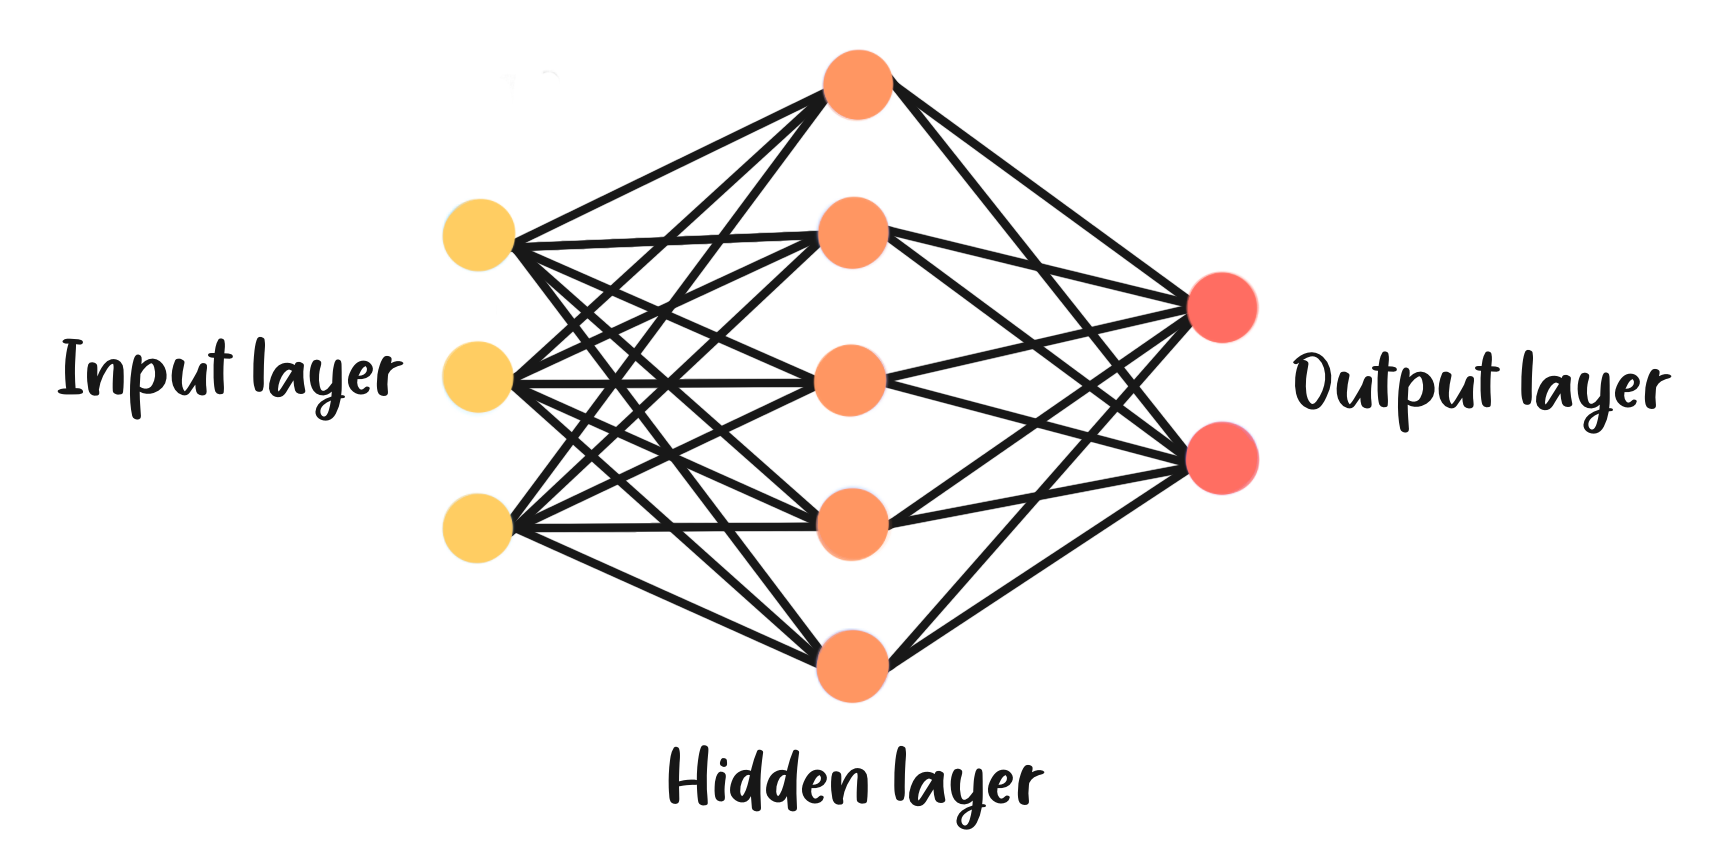
\includegraphics[width=10cm]{Images/mlp.png}
    \caption{Multi-Layer Perceptron}
    \label{fig:mlp}
\end{figure}
An input layer, one or more hidden layers, and an output layer are the minimum number of nodes that make up a \gls{mlp} feedforward artificial neural network type (Figure \ref{fig:mlp}).
All nodes in these layers—aside from those in the input layer—are linked using a specific weight and employ a nonlinear activation function.
Because of its nonlinearity, the network may learn and carry out more complicated tasks as well as represent intricate connections between the input and output.
A \gls{mlp} model is trained by comparing its output to the expected output and propagating errors back through the network to alter the weights. 
This process is known as backpropagation. \\\cite{haykin_2014_neural}

\paragraph{Convolutional Neural Networks}
\nocite{ibm_2023_what_cnn}
\nocite{mishra_2020_convolutional}
\nocite{mandal_2021_cnn}
\nocite{saha_2018_a}
\gls{cnns} are a family of deep learning algorithms that are mostly utilized for processing input that has a grid structure, like images. \cite{yamashita_2018_convolutional}
\\
\begin{figure}[!ht]
    \centering
    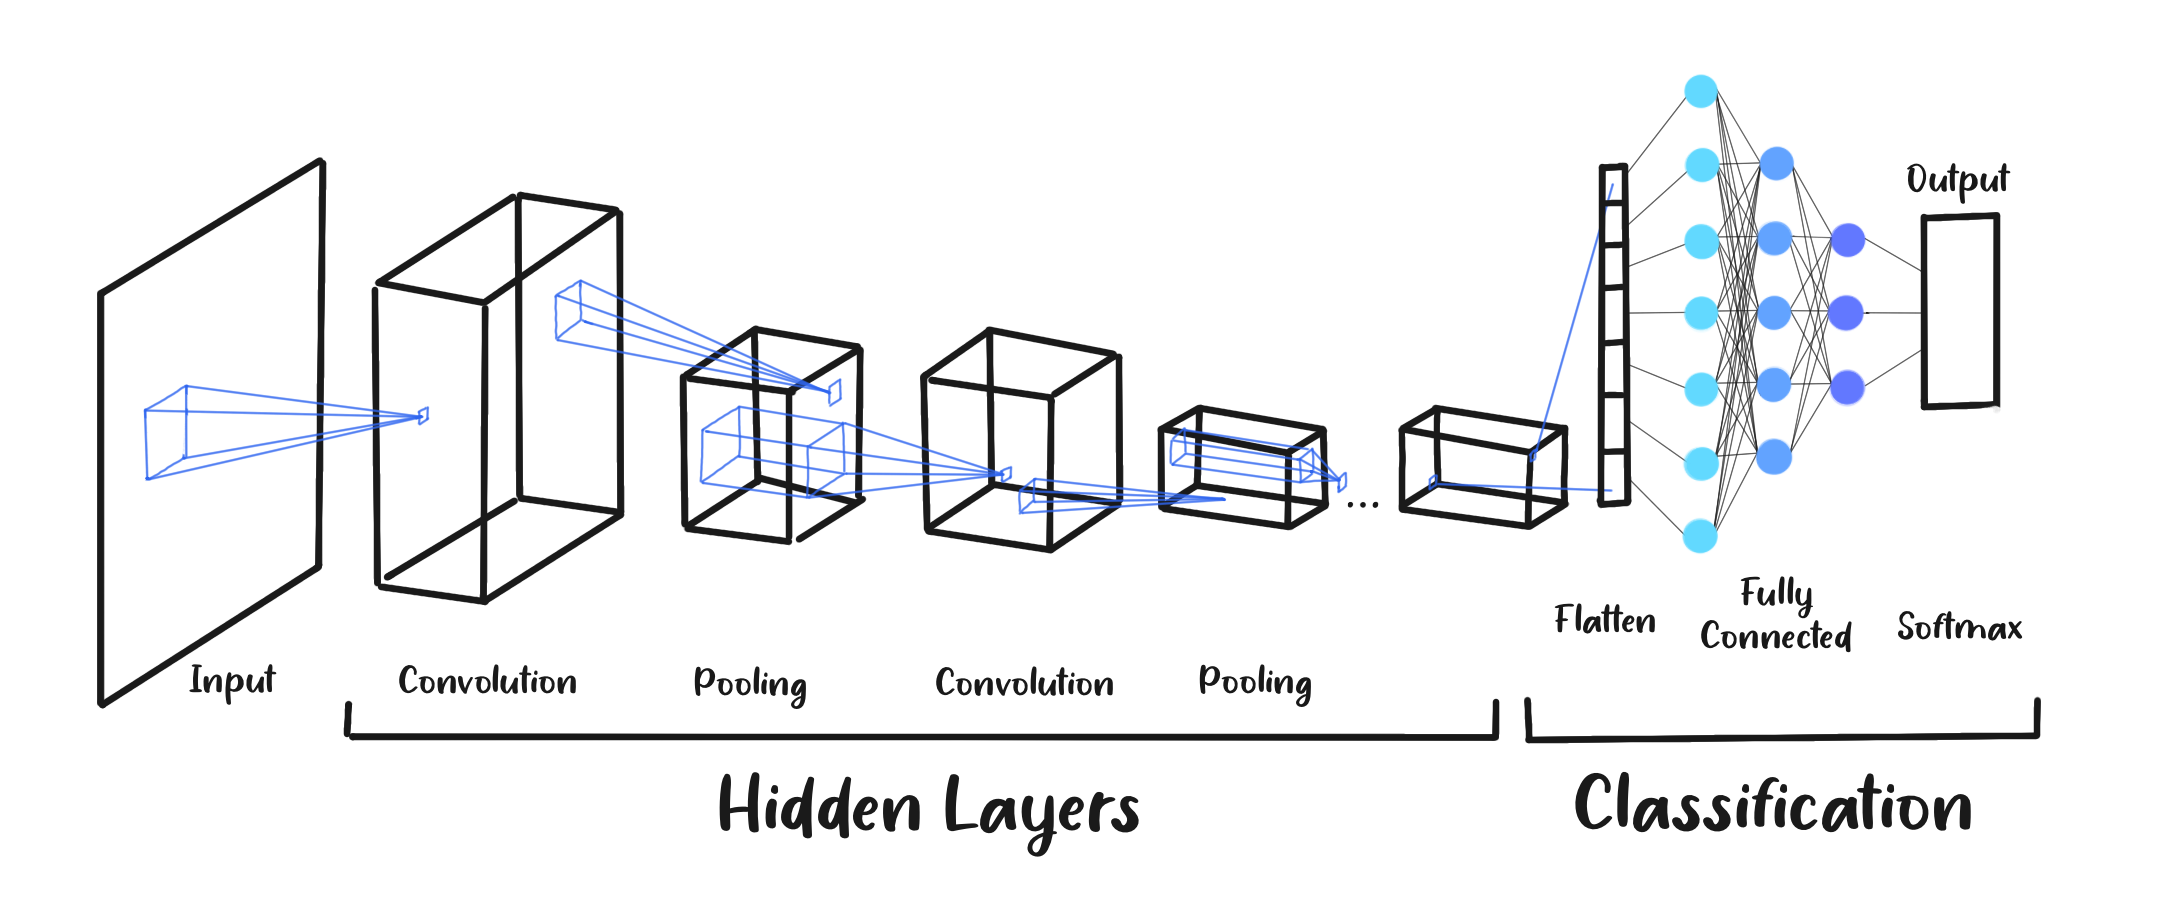
\includegraphics[width=16cm]{Images/cnns.png}
    \caption{Convolutional Neural Networks}
    \label{fig:cnns}
\end{figure}
\\
\indent \gls{cnns} are designed to adaptively learn spatial hierarchies of features from the data. 
This learning process includes convolution layers, pooling layers, flatten layer, and fully connected layers.
By applying filters, also known as kernels, to the input, these layers carry out the convolution process and produce feature maps. 
Local elements like textures and edges are captured throughout this procedure.
Pooling layers, which come after convolutional layers, help to reduce the number of parameters and computation in the network by reducing the spatial dimensions (width and height) of the input volume. 
\\
\indent The features from the input image are retrieved by the convolutional and pooling layers, and the next stage is to categorize the features which is done in flatten layer.
The feature maps are converted into a one-dimensional vector in the flatten layer, which is necessary for fully connected layers.
The flattened vector is then fed into the fully connected layers (which resemble the standard neural network layers with fully connected nodes) for the classification task. 
These fully connected layers divide the image into discrete groups based on the high-level characteristics found in the preceding levels.
\\
\indent The last layer of layers in the network architecture play the crucial job of generating the output.
The output layer typically uses a softmax activation function in multi-class classification settings to translate the network's raw output into probabilities given to each class. 
The output node with the highest probability is then chosen to determine the anticipated class.
\\
\section{Facial Emotion Recognition}
Human emotions can be inferred from facial expressions. 
Deciphering these signs of emotion has become a popular research topic in the fields of Human Computer Interaction and Psychology. \cite{vemou_2021_facial}
The development of \gls{fer} technology has been significantly aided by technological advancements, particularly with the introduction of \gls{ml} and Pattern Recognition.
\\
\begin{figure}[!ht]
    \centering
    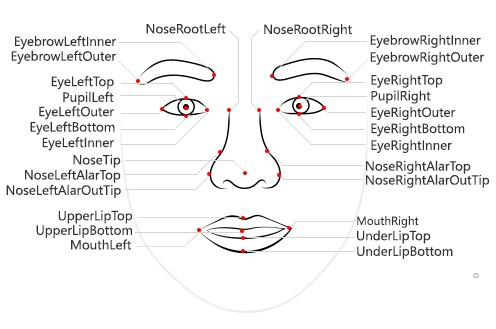
\includegraphics[width=10cm]{Images/landmarks.jpg}
    \caption{Facial Landmarks} \footnotesize{Image from \cite{patrickfarley_2023_face}}
    \label{fig:facial_landmark}
\end{figure}
\\
\indent \gls{fer} is a broad field that intersects with Computer Science, \gls{ai}, Psychology and other fields. 
It involves analyzing a person's facial expressions in still images and videos in order to determine their emotional state. 
A three-step approach is used in the methodology: face detection, facial expression identification, and categorization of the expression into a certain emotional state. 
Facial landmark (Figure \ref{fig:facial_landmark}) detection and analysis of changes in their positions are key components of this complex process. 
\gls{fer} attempts to offer insights into people's emotional experiences by identifying muscular contractions linked to various emotions from visual clues found in facial expressions.
\\
\begin{figure}[!ht]
    \centering
    \subfloat[\centering Confusion Matrix for k-NN Classifier \label{subfig:knn-tarnowski}]{{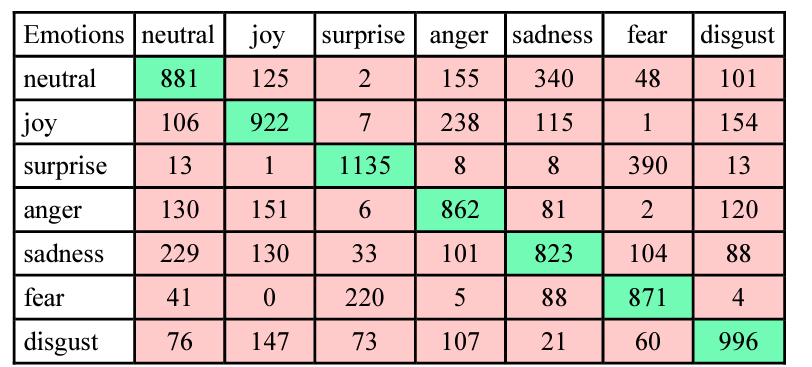
\includegraphics[width=7cm]{Images/fer1stknn.png}}}%
    \qquad
    \subfloat[\centering Consfusion Matrix for MLP Classifier \label{subfig:mlp-tarnowski}]{{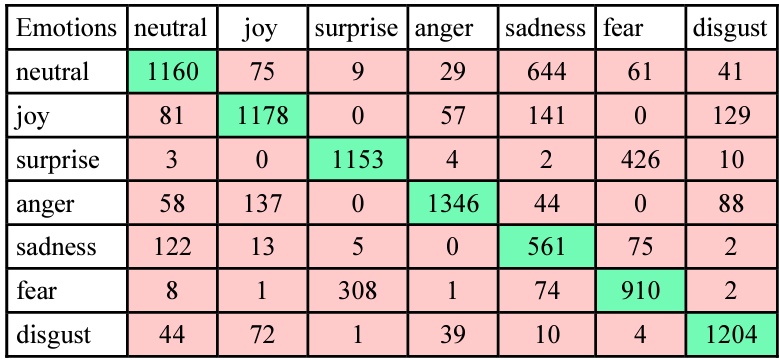
\includegraphics[width=6.7cm]{Images/fer1stmlp.png}}}%
    \vspace{0.5cm}
    \\
    \scriptsize{Tables from \cite{tarnowski_2017_emotion}}
\end{figure}
\\
\indent As stated by Tarnowski et al. (2017), the creative feature extraction from facial expressions using coefficients that detailed aspects of emotional states is what makes the research successful.
They distinguished between seven different emotional states: happiness, sorrow, surprise, wrath, fear, and contempt, as well as the more subdued displays of neutrality. 
For featre computation, they employed a three-dimensional facial model as an alternative to conventional two-dimensional approaches. 
This enables them to collect more detailed and subtle data, which may improve the accuracy of identifying emotions. 
On top of that, they used the MLP neural network and the \gls{knn} classifier to classify each emotional state. 
According to their research and comparative analysis, the MLP is more accurate than the \gls{knn} in classifying emotional states, with a 73\% classification accuracy compare to a 63\% accuracy for \gls{knn} \cite{tarnowski_2017_emotion}.
\\
\indent Mellouk et al. (2020) showed in their study that \gls{fer} may be achieved with great accuracy and effectiveness by utilizing deep learning techniques.
They provided a thorough analysis of multiple \gls{fer} databases, emphasizing their diversity in terms of picture, video content, lightning circumstances, and demographic variances—all of which are important determinants of \gls{fer} performance—in order to guarantee the credibly of the results.
\\
\indent Traditional facial recognition techniques included manually defining and extracting features from facial photos, a procedure that was frequently less flexible and efficient. 
Examples of these techniques include Local Binary Patterns (LBP), Facial Action Coding System (FACS), Local Directional Patterns (LDA), and Gabor wavelet. 
\gls{cnns} and LSTMs can automatically extract and learn complex patterns from facial data, according to Mellouk et al., which will improve the reliability and accuracy of emotion recognition. 
Furthermore, the difficulties that traditional approaches faced—such as variances in facial characteristics due to diverse demographics, occlusions, and data diversity—are resolved with the use of deep learning, increasing their versatility and effectiveness.
The study also examines preprocessing methods including image scaling, cropping, normalization, and data augmentation that are crucial for improving the accuracy of these deep learning models.
\\
\indent With the help of deep learning and the preprocessing techniques they found, the outcome demonstrates proficiency in accurately classifying the fundamental emotions, with some models reaching over 90\% accuracy under specific circumstances \cite{mellouk_2020_facial}. 
It indicates that as machines improve at deciphering human emotions, interactions between humans and machines may become more intuitive and natural.
\\
\begin{figure}[!ht]
    \centering
    \subfloat[\centering Accuracy variation with 32 Filters and 8 kernel size for Model 1 \label{subfig:new_cnn1}]{{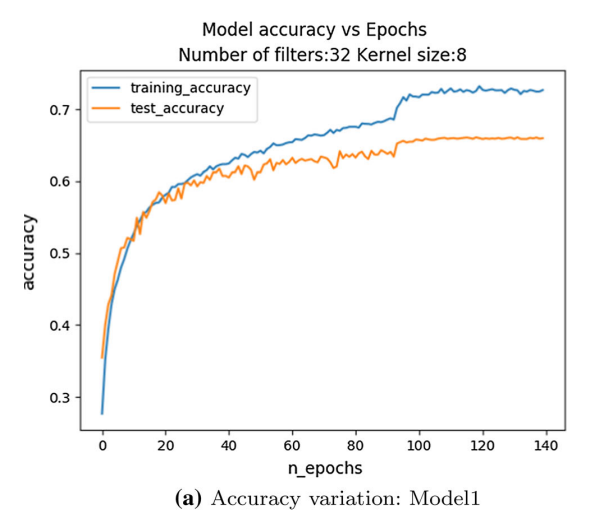
\includegraphics[width=6.8cm]{Images/new_cnn_model1.png}}}%
    \qquad
    \subfloat[\centering Accuracy variation with 32 Filters and 8 kernel size for Model 2 \label{subfig:new_cnn2}]{{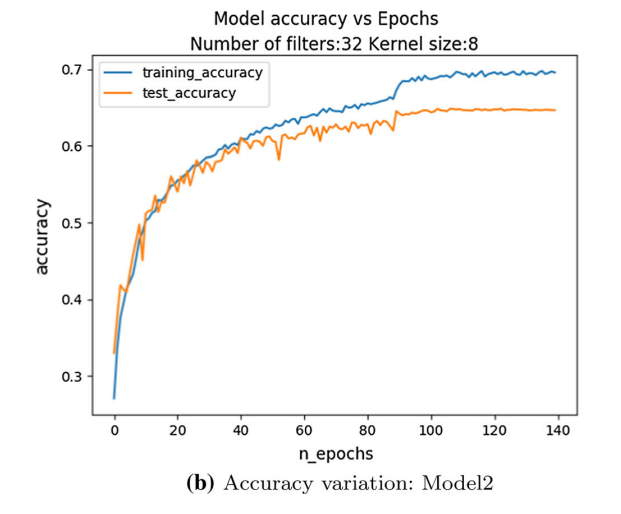
\includegraphics[width=7cm]{Images/new_cnn_model2.png}}}%
    \vspace{0.5cm}
    \\
    \scriptsize{Graphs from \cite{agrawal_2019_using}}
\end{figure}
\\
\indent Based on the findings of Agrawal et al.'s work, the kernel size and the number of filters significantly impact \gls{cnns} accuracy.
Using the FER-2013 dataset as their primary emphasis, two CNN architectures is put forth after a thorough analysis of various kernel sizes and filter counts.
To find the optimal set of parameters that could yield the best convergence and accuracy, Agrawal et al. ran tests with the combination of 6 different kernel sizes (2, 4, 8, ..., 64) and 8 different number of filters (2, 4, 8, ..., 256). 
They discovered that when network depth increased, a network with 32 filters and an 8 kernel size demonstrated a discernible gain in accuracy (Figure \ref{subfig:new_cnn1}, Figure \ref{subfig:new_cnn2}).
\\
\begin{figure}[!ht]
    \centering
    \subfloat[\centering Confusion Matrix for Model 1 \label{subfig:new_cm1}]{{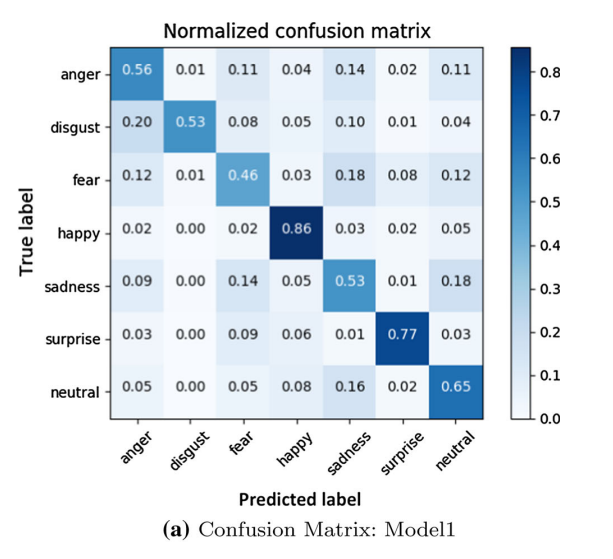
\includegraphics[width=7cm]{Images/new_cnn_cm_1.png}}}%
    \qquad
    \subfloat[\centering Confusion Matrix for Model 2 \label{subfig:new_cm2}]{{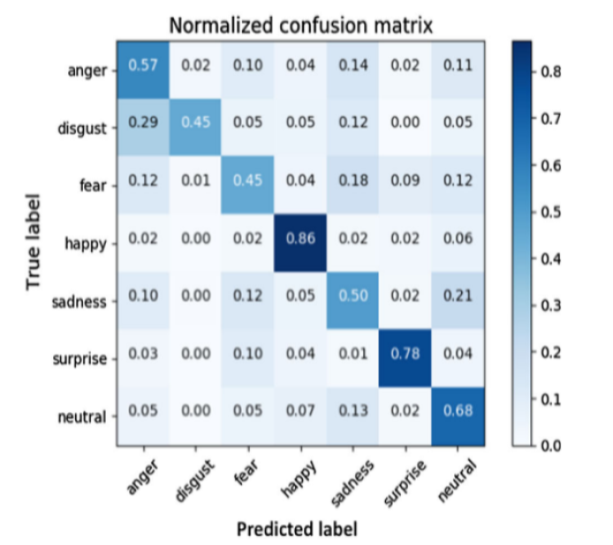
\includegraphics[width=7cm]{Images/new_cnn_cm_2.png}}}%
    \vspace{0.5cm}
    \\
    \scriptsize{Graphs from \cite{agrawal_2019_using}}
\end{figure}
\\
\indent Even while Model 2 is simpler due to its constant kernel size, lack of dropout layers, and fully connected layers, it was nevertheless able to achieve an accuracy of 65\% on the FER-2013 dataset, which is comparable to human performance \cite{agrawal_2019_using}.
Furthermore, in comparison with other emotions, the proposed models were able to categorize happiness and surprise with a higher degree of accuracy, which is consistent with people's challenges in picking out distinct emotions (Figure \ref{subfig:new_cm1}, Figure \ref{subfig:new_cm2}).
\\
\begin{figure}[!ht]
    \centering
    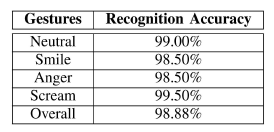
\includegraphics[width=6cm]{Images/lr_result.png}
    \caption{Linear Regression Classification Accuracies Table} \footnotesize{Table from \cite{naseem_2010_linear}}
    \label{fig:lrc_result}
\end{figure}
\\
\indent A pivotal study by Naseem et al. (2010) incorporates the analysis of facial expressions, recognizing them as crucial variations in appearance induced by internal emotions or social communications.
In order to evaluate their \gls{lr} Classification approach, they therefore took into account occlusion modes, brightness changes, and expressions such as scream, smile, rage, and neutral
Notably, the \gls{lr} Classification algorithm showed an excellent recognition accuracy for all facial expressions tested, averaging 98.88\% in a 100D feature space (Figure \ref{fig:lrc_result}). 
For the screaming expression, the algorithm outperformed other accuracies by achieving an accuracy of 99.5\% (Figure \ref{fig:lrc_result}).
This great accuracy demonstrates the reliability and efficacy of the LRC approach in handling a wide range of facial emotions.
\\
\begin{figure}[!ht]
    \centering
    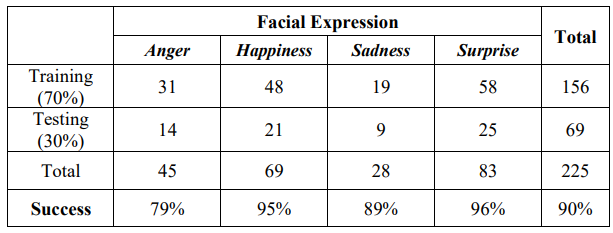
\includegraphics[width=10cm]{Images/rf_result.png}
    \caption{Random Forest Classification Accuracy} \footnotesize{Table from \cite{munasinghe_2018_facial}}
    \label{fig:rf_result}
\end{figure}
\\
\indent According to Munasinghe (2018), \gls{rf} Classifier are capable of handling facial expression variability well and without overfitting.
Also, the researcher asserts that facial landmarks (Figure \ref{fig:facial_landmark}) provide an accurate feature extraction capability that capture subtle changes in facial emotions.
A facial feature vector obtained from these landmarks and normalized to reduce variance in face size is used to discern emotions with a \gls{rf} Classifier.
With the aid of feature vector, the \gls{rf} Classifier achieved an average success rate of 90\% in classifying four different emotions: anger, happiness, sadness, and surprise (Figure \ref{fig:rf_result}).
\\
\begin{figure}[!ht]
    \centering
    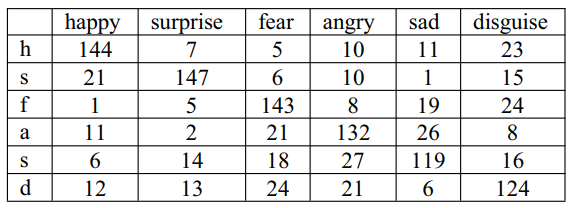
\includegraphics[width=10cm]{Images/svm_result.png}
    \caption{Support Vector Machine Accuracy} \footnotesize{Table from \cite{xia_2014_facial}}
    \label{fig:svm_result}
\end{figure}
\\
\indent Li Xia (2014) presents a unique method of facial emotion detection that employs multi-classification \gls{svm}.
The study proposes a two-on-two classification method which is an innovative approach to overcome the limitations of traditional classification methods like one-against-one (classifier is trained for each pair of classes) and one-against-the-rest (classifier is trained against all other classes combined).
With this novel method, the classification process is faster with fewer sub-classifiers and reduced classification errors.
The results of this study were impressive, showing the classifier in this investigation demonstrated a high average recognition rate of 92.7\% when six distinct emotions were considered, including happiness, surprise, anger, fear, disgust, and sadness. 
\\
\section{Music Recommendation based on FER}
From Chakrapani et al.'s approach, music recommendation system with deep learning algorithm could enhance the listening experience by accurately detect and interpret the user's emotions.
This is achieved by using \gls{cnns} to analyze the user's age, gender, and facial emotion. Based on these data, the system would cater to the user's preferences and present mood.
To ascertain the user's emotional state, they used the webcam to take pictures of the user and then processed the image using the \gls{cnns} models.
The system then provided tailored music recommendations based on the predictions generated by the \gls{cnns} models. 
This approach offers a creative and user-centric alternative for music selection based on emotional cues while streamlining playlist construction and management.\cite{mrchakrapanids_2023_music}
\\
\indent Additionally, Athavle et al. discovered that using \gls{cnns} model helps a music recommendation system to accurately detect emotions and subsequently recommend music that aligns with the user's mood.
They train a \gls{cnns} model for emotion detection in their work. 
While maintaining great precision, this method lowers total system costs and computing time.
The system uses real-time emotion detection to work, and then sends the data to the \gls{cnns} model to classify the user's emotions. 
An appropriate playlist will be recommended as soon as the technology determines the user's current feeling, making the user experience engaging and responsive.
In order to guarantee optimal classification accuracy and efficacy, they employed categorial cross-entropy as a loss function to manage missing and anomalous values inside the FER2013 dataset.
Despite their result being less accurate than Chakrapani et al.'s work (71\%), it nevertheless shows that the model is effective and trustworthy in identifying emotions from facial expressions. \cite{athavle_2021_music}
